\documentclass[11pt]{article}

\usepackage{sectsty}
\usepackage{graphicx}
\usepackage{amsmath, amssymb, amsfonts, amsthm}

% Margins
\topmargin=-0.45in
\evensidemargin=0in
\oddsidemargin=0in
\textwidth=6.5in
\textheight=9.0in
\headsep=0.25in
\DeclareMathOperator{\erf}{erf}
\DeclareMathOperator{\erfc}{erfc}

\title{MHIT36}
\author{Alessio Roccon}
\date{\today}

\begin{document}
\maketitle	
\pagebreak

% Optional TOC
% \tableofcontents
% \pagebreak

%--Paper--
\part{Formulation}

\section{Governing equations}

A first tentative try of the governing equation for boiling flow reads as [adapted from Karniadakis]:
\begin{equation}
\nabla \cdot  {\bf u} =  0\, ,
\end{equation}
%where $\rho_r=\rho_v/ \rho_l$.

For the Navier-Stokes equations, by assuming constant viscosity and density, the following equation can be derived:
\begin{equation}
\frac{\partial {\bf u}}{\partial t} + \nabla \cdot ({\bf u}{\bf u})= - \frac{ \nabla p}{\rho}  +  \nu \nabla^2 {\bf u}  + \frac{ \sigma}{\rho} k {\bf n} + {\bf f}
\end{equation}

The interface is captured using a second-order phase field method:
\begin{equation}
\frac{\partial \phi}{\partial t} +  \nabla \cdot ( {{\bf u} \phi }) = \nabla \cdot \left[ \gamma \left (\epsilon \nabla \phi  - \phi (1-\phi) \frac{\nabla \phi}{|\nabla \phi|}  \right) \right] \, ,
\end{equation}
The first two terms at the right hand side are the classical sharpening and diffusive terms.

Likewise, $\epsilon$ should be set equal to: 
\begin{equation}
\epsilon > 0.5 \Delta x
\end{equation}

\section{Numerical implementation}


\subsection{NS solver}

Projection-correction + Poisson solver based on 3D FFT along all directions
The first step is to rewrite the NS equations as follows:
\begin{equation}
\frac{\partial {\bf u}}{\partial t} = - \nabla \cdot ({\bf u}{\bf u}) - \frac{ \nabla p}{\rho}  +  \nu \nabla^2 {\bf u}  + \frac{ \sigma}{\rho} k {\bf n} + {\bf f}
\end{equation}
Then, we perform the projection step where the right hand side is computed using the right hand side evaluated at time step $n$.
As pressure is not known, the pressure gradient term is ignored during this first step.
Discretizing in time the equation and ignoring the pressure gradient term as well as the surface tension term (for simplicity), we have:
\begin{equation}
\frac{ {\bf u^* - u^n}}{\Delta t} = - \nabla \cdot ({\bf u}{\bf u})^n +  \nu \nabla^2 {\bf u}^n  + {\bf f}^n
\end{equation}
Thus, we can obtain the provisional field $\bf u^*$ as follows:
\begin{equation}
{\bf u^*} = {\bf u}^n + \Delta t (  - \nabla \cdot (  {\bf u}{\bf u})^n +  \nu \nabla^2 {\bf u}^n  + {\bf f}^n)\, ,
\end{equation}
This provisional field (result of the the projection step) is however not divergence free and we must correct so to obtained the filed $n+1$, which should be divergence free.
We can correct the field as follows:
\begin{equation}
{\bf u^{n+1}} = {\bf u}^* - \frac{\Delta t}{\rho} \nabla p^{n+1}\, ,
\end{equation}
where this equation comes from:
\begin{equation}
\frac{ {\bf u^{n+1} - u^*}}{\Delta t} = - \frac{1}{\rho} \nabla p^{n+1}\, 
\end{equation}
to make clear that the algorithm is really just an operator splitting approach in which one considers the convective and viscous forces (in the first half step) and the pressure forces (in the second half step) separately.
Computing the right-hand side of the second half step requires knowledge of the pressure at $n+1$.
This is obtained by taking the divergence and requiring that the new flow field $n+1$ is divergence free.
\begin{equation}
\nabla^2 p^{n+1} = \frac{\rho}{\Delta t} \nabla \cdot {\bf u^*}\, ,
\end{equation}
This is a Poisson equation (most expensive part of the entire scheme), which should be solved using FFT-based solvers (present case) or iterative/multigrid methods. 


\subsection{CAC solver}

Euler explicit + FD2.
Solver is totally explicit 

\subsection{Forcing of turbulence}

When performing direct numerical simulations of homogeneous turbulence, one would like to force turbulence for two reasons. 
First, it permits to reach higher Reynolds numbers than in freely decaying turbulence. 
Second, under some assumptions, statistics can be obtained with time-averaging rather than ensemble averaging, which would be very costly considering the fact that refined statistics require a large number of samples. 
To study statistically stationary turbulence, many velocity forcing schemes have been used so far in numerical simulations. 
In homogeneous spectral simulations, large-scale forcing methods consist in providing energy to the low wavenumber modes, which is consistent with the concept of Richardson cascade. 
For example, considering a working an external force $\bf f$ which is a linear combination of sines and cosines with wavevectors of modulus lesser than or equal to $k_f$, the forcing contribution in both
Craya’s equation and energy spectral density equation vanishes at wave numbers greater than $k_F$.
Therefore, in statistically stationary turbulence, this external force feeds low wavenumbers and then part of this energy is transferred to larger wavenumbers through the nonlinear term.

\subsubsection{ABC forcing scheme}
The ABC forcing is defined as follows:
\begin{equation}
{\bf f} = [B \cos (k_F y) + C \sin (k_F z) ]{\bf i} \\ + [C \cos (k_F z)+ A \sin (k_F x) ]{\bf j} + [A \cos (k_F x) + B \sin (k_F y)] {\bf k}\, ,
\end{equation}
for a given large scale wavenumber $k_F$. 
Since ABC is an eigenfunction of the curl operator with eigenvalue $k_F$, the corresponding contribution in the helicity equation is nonzero and thus the ABC forcing injects helicity, in addition to energy, in the flow [See Intermittency in the isotropic component of helical and non-helical turbulent flows]
Usually $A=B=C=1$, other possible choice: $A=0.9$, $B=1$ and $C=0.9$, see paper listed above.

\subsubsection{TG forcing scheme}
The TG forcing is defined as follows:
\begin{equation}
{\bf f} = f_0 [ \sin (k_F x)  \cos (k_F y) \cos(k_F z) {\bf i}  - \cos (k_F x) \sin (k_F y) \sin (k_F z) {\bf j}] \, ,
\end{equation}
Here $f_0$ is the forcing amplitude, which can be set to have in the turbulent steady state all runs with r.m.s. velocities near unity.

\subsubsection{Lundgren scheme}
A local force proportional to the local velocity is imposed on the fluid:
\begin{equation}
{\bf f} = A_f {\bf u}\, ,
\end{equation}
where the coefficient $A_f$ is calculated as follows:
\begin{equation}
A_f = \frac{\epsilon}{3 \langle u_{rms}^2 \rangle }
\end{equation}
To generate turbulence, the Lundgren forcing requires a non- zero initial velocity field



\subsubsection{Mallouppas-type force}

The forcing scheme proposed by Mallouppas, George, and van Wachem reads as follows:
\begin{equation}
{\bf f} = \frac{\rho}{\Delta t} \frac{\sqrt{k_{wanted}} - \sqrt{k_{computed}} }{\sqrt{k_{wanted}}}{\bf u}_{triggered}
\end{equation}
where $\Delta t$ is the time step, $k_{wanted}$ is the specified turbulent kinetic energy, $k_{computed}$ is the computed turbulence kinetic energy of the domain, and ${\bf u}_triggered$ is a pseudo-velocity field, which is
carefully chosen and synthesized from a model spectrum.
Following the explanation of Cant we use the procedure proposed by Kwak, Reynolds, and Ferziger to generate a divergence-free isotropic velocity field corresponding to a given energy spectrum. 
The Batchelor–Townsend energy spectrum was used as an initial energy spectrum to create the velocity field. 
This spectrum represents the later stages of the decay of grid turbulence and is expressed as follows:
Code to generate a synthetic velocity field corresponding to the Batchelor–Townsend energy spectrum available here https://web.stanford.edu/$\sim$hjbae/CBC.






\subsection{Simulation setup}
The governing equations are solved in a triple-periodic domain with length $L=2 \pi$.
The variable are defined on a staggered grid with scalars (pressure and phase-field variables) defined at cell center (empty dot in figure~1) and velocity components at cell faces (full circles in figure~1).






\begin{figure}[!t]
\centering
    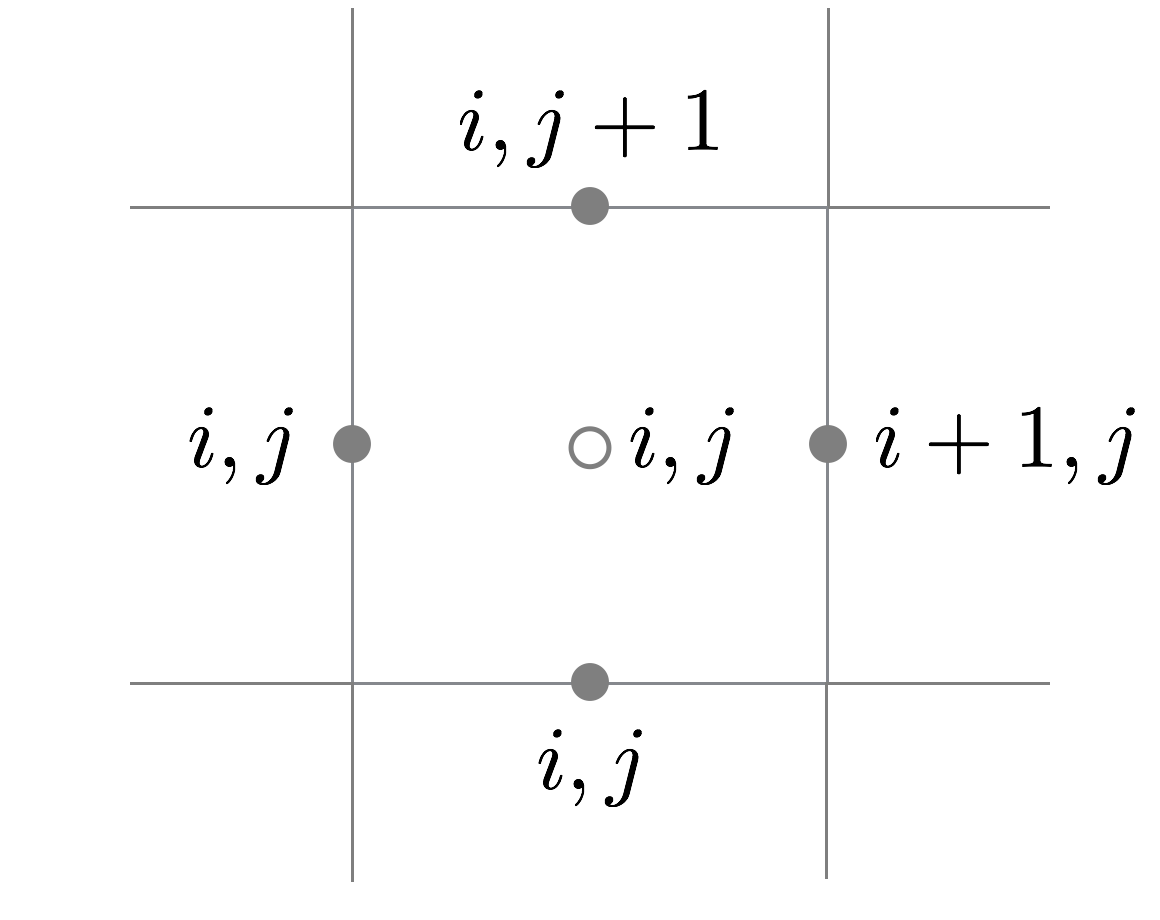
\includegraphics[width=0.3\textwidth]{staggered_2.png} 
    \caption{Staggered grid in 2D and examples of node numbering used in MHIT36.}
    \label{fig1}
\end{figure}



\end{document}



